\chapter{GIAO TIẾP I2C}
\section{Giới thiệu chung}
\subsection{Yêu cầu}Viết chương trình giao tiếp I2C giữa vi điều khiển PIC 16F887 với các module có chuẩn giao tiếp I2C.
\subsection{Chuẩn I2C}
Chuẩn I2C là chuẩn giao tiếp 2 dây là \verb|Serial Data (SDA)| (truyền dữ liệu 2 hướng) và \verb|Serial Clock (SCL)| (truyền xung đồng hồ theo một hướng).\\

Cách kết nối: chân \verb|SDA, SCL| của module lần lượt nối đến chân \verb|SDA, SCL| của vi điều khiển PIC 16F887. Ta có thể kết nối điều khiển nhiều thiết bị I2C với nhau thông qua 2 chân \verb|SDA| và \verb|SCL| của vi điều khiển. Mỗi thiết bị I2C sẽ được phân biệt bằng một \emph{địa chỉ duy nhất} \verb|address| hoặc \emph{quan hệ chủ tớ} \verb|master - slave|.
\section{Giao tiếp chuẩn I2C với CCS}
Để giao tiếp ta dùng khai báo và các lệnh sau:
\begin{itemize}
\item Khai báo: \verb|#use I2C(mode, speed, SDA = PIN_C4, SLC = PIN_C3)|, với:
\begin{itemize}
\item \verb|mode|: \verb|master| hoặc \verb|slave|.
\item \verb|speed|: \verb|slow| $\left({100kHz}\right)$ hoặc \verb|fast| $\left({400kHz}\right)$.
\item Trên PIC 16F887, chân \verb|C4| và chân \verb|C3| lần lượt là chân \verb|SDA| và \verb|SCL|.
\end{itemize}
\item Các hàm giao tiếp được CCS định nghĩa:
\begin{itemize}
\item \verb|I2C_ISR_STATE()|: Thông báo trạng thái giao tiếp I2C.
\item \verb|I2C_START()|: Tạo điều kiện \verb|START|.
\item \verb|I2C_STOP()|: Tạo điều kiện \verb|STOP|.
\item \verb|I2C_READ(mode)|: Đọc giá trị \verb|8 bit| thiết bị I2C. Với \verb|mode = 0| (không chỉ ra \verb|ACK|) và \verb|mode = 1| (chỉ ra \verb|ACK|)
\item \verb|I2C_WRITE(Device_address)|: Ghi giá trị \verb|8 bit| đến thiết bị I2C.
\end{itemize}
\item[$\ast$] Để hiểu rõ hơn các hàm này, có thể xem trong phần \verb|Help| của CCS.
\end{itemize}
\section{Bài tập}
\subsection{Bài tập 6.1}\label{Ex:6-1}
\paragraph{Yêu cầu}Viết chương trình đọc giá trị nhiệt độ từ cảm biến nhiệt TC 47 và hiển thị lên LCD 16x02.
\paragraph{Hướng giải quyết}
\begin{itemize}
\item Xác định chế độ truyền là \verb|Master| (quan hệ chủ -- tớ $\longleftrightarrow$ PIC (chủ) -- TC74 (tớ)).
\item Xác định địa chỉ của thiết bị I2C TC74 là: \verb|0x48| (Do thiết bị thực tập là TC74A0-5.0VAT, tùy dòng IC mà chúng ta xác định địa chỉ cho thích hợp, \textit{tham khảo trang 9 của datasheet \footnote{http://www.alldatasheet.com/} TC74}). %thêm số 0 vào cuối 7 bit trong trang 9 để được địa chỉ của thiết bị TC74).
\item Để giao tiếp với ngoại vi chuẩn I2C theo quan hệ chủ tớ, ta thực hiện như sau:
\begin{itemize}
\item Thiết bị chủ (PIC) tạo điều kiện \verb|Start|: \verb|i2c_start();|
\item Thiết bị chủ gửi địa chỉ của thiết bị tớ cùng với 1 bit 0, tức là gửi địa chỉ \verb|0x90| (\verb|0x48 = 1001000|, thêm bit 0 vào cuối: \verb|1001000 0 = 0x90|), dùng lệnh: \verb|i2c_write(0x90);| và đợi xung \verb|ACK| phản hồi từ thiết bị tớ (phần này đã giải thích tại sao phải thêm số 0 vào cuối 7 bit địa chỉ ở ý trên).
\item Khi thiết bị tớ đã nhận được đúng địa chỉ của nó (phản hồi xung \verb|ACK|), thiết bị chủ gửi lệnh thông báo truy cập vào thanh ghi đọc nhiệt độ - lệnh \verb|00h|, dùng lệnh: \verb|i2c_write(0x00);| (phần lệnh của TC74 được mô tả ở trang 8 trong datasheet).
\item Ta đã hoàn thành việc \textit{gửi yêu cầu đọc nhiệt độ} từ thiết bị tớ -- TC74, tiếp theo là thiết bị chủ (PIC) sẽ \textit{đọc giá trị nhiệt độ} từ thiết tớ (TC74).
\item Tạo lại điều kiện \verb|Start| để thực hiện giao tiếp mới: \verb|i2c_start();|
\item Thiết bị chủ gửi địa chỉ của thiết bị tớ cùng với bit 1 (lấy địa chỉ thiết bị I2C thêm vào bit 1: \verb|1001000 1 = 0x91|), dùng lệnh: \verb|i2c_write(0x91);|
\item Phần còn lại là đọc giá trị nhiệt độ từ thiết bị tớ, thiết bị chủ gửi xung \verb|Not-ACK| dùng lệnh: \verb|i2c_read(0);| (giá trị là số nguyên 8 bit).
\item Tạo điều kiện \verb|Stop|: \verb|i2c_stop();| để kết thúc quá trình giao tiếp.
\item Để giao tiếp được nhiều lần, ta thực hiện vòng lặp \verb|while| để lặp lại quá trình này (từ lệnh \verb|i2c_start();| đến \verb|i2c_stop();|).
\end{itemize}
\item Chúng ta lấy được giá trị nhiệt độ từ cảm biến TC74 và gửi lên LCD để quan sát.
\item Phần mô phỏng chương trình với phần mềm Protues em trình bày trong phần \textit{phục lục trang \pageref{def:TC74}}.
\item[$\ast$] Khi làm phần cứng, cần mắc thêm 2 điện trở \verb|pullup| lên nguồn.
\item[$\ast$] Ngoài cách giải thích trên, chúng ta có thể tham khảo cách giải thích khác trong phần chú thích \ref{note:TC74} ở bên dưới\footnote{http://embedded-lab.com/blog/using-tc74-microchip-thermal-sensor-for-temperature-measurement/\label{note:TC74}}.
\end{itemize}
\section*{Sơ đồ mạch}
\begin{figure}[!h]
\begin{center}
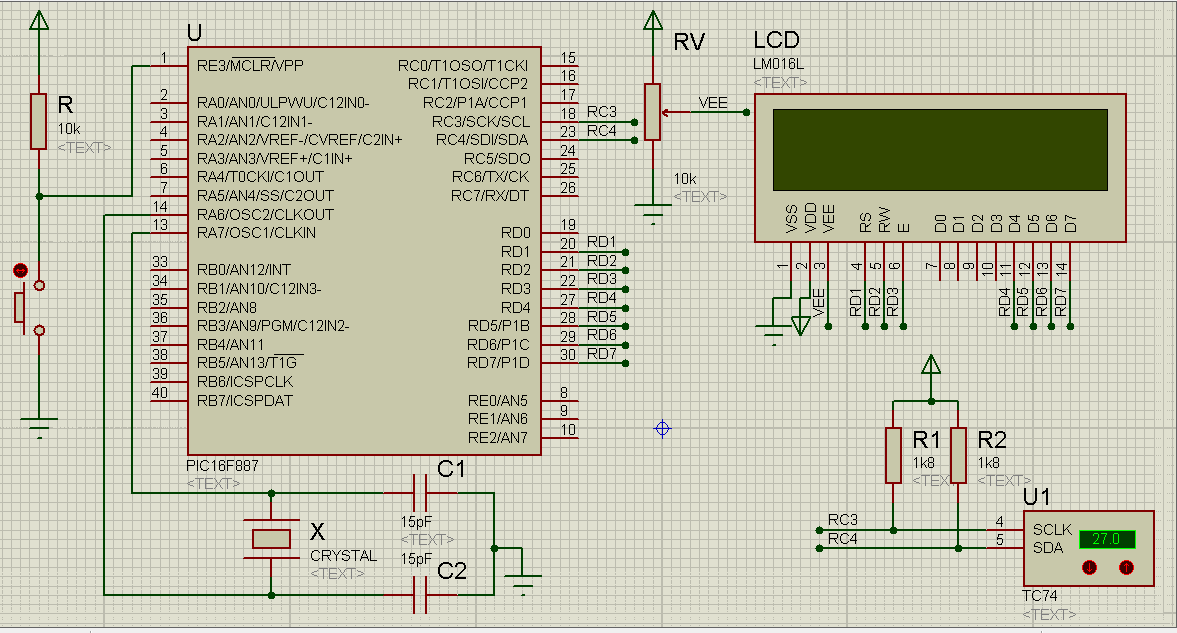
\includegraphics[scale=0.45]{bai-6/image/BAI-6-1}
\end{center}
\caption{Mạch đọc giá trị nhiệt độ từ IC TC74}
\end{figure}
\newpage
\subsection*{Chương trình 17}
\lstinputlisting[language=C]{BAI-6-1.C}
\subsection{Bài tập 6.2}
\label{Ex:ds3231-1}
\paragraph{Yêu cầu}Viết chương trình đọc giá trị thời gian từ IC DS1307 và hiển thị lên LCD 16x02.
\paragraph{Hướng giải quyết}Do không có IC DS1307 nên em thay thế bằng phần cứng khác là module RTC DS3231.
\begin{itemize}
\item[$\ast$] So với IC DS1307 thì IC DS3231 có thời gian chạy chính xác hơn. Module RTC DS3231 ngoài chức năng lấy thời gian thực, nó còn chức năng đo được giá trị nhiệt độ.
\item Chúng ta quan tâm đến các địa chỉ sau:
\begin{itemize}
\item Địa chỉ của thiết bị I2C là \verb|0x68|.
\item Địa chỉ của các thanh ghi lưu giá trị thời gian:
\begin{table}[!h]
\begin{center}
\begin{tabular}{|l|c|l|c|}\hline
\textit{Thanh ghi} & \textit{Địa chỉ} & \textit{Thanh ghi} & \textit{Địa chỉ}\\ \hline
\verb|secondREG| & \verb|0x00| & \verb|dayREG| & \verb|0x03| \\ \hline
\verb|minuteREG| & \verb|0x01| & \verb|dateREG| & \verb|0x04| \\ \hline
\verb|hourREG| & \verb|0x02| & \verb|monthREG| & \verb|0x05| \\ \hline
& & \verb|yearREG| & \verb|0x06| \\ \hline
\end{tabular}
\end{center}
\caption{Địa chỉ thanh ghi thời gian của IC DS3231}
\end{table}
\item Cài đặt định dạng thời gian hiển thị:
\begin{table}[!h]
\begin{center}
\begin{tabular}{|c|c|c|c|}\hline
\textit{Định dạng} & \textit{Cài đặt} & \textit{Định dạng} & \textit{Cài đặt} \\ \hline
\verb|_24_hour_format| & \verb|0| & \verb|am| & \verb|0| \\ \hline
\verb|_12_hour_format| & \verb|1| & \verb|pm| & \verb|1| \\ \hline
\end{tabular}
\end{center}
\caption{Cài đặt định dạng thời gian hiển thị}
\end{table}
\end{itemize}
\item Giá trị lưu trong thanh ghi ở dạng \verb|BCD|. Nên muốn ghi giá trị vào thanh ghi cần chuyển sang mã \verb|BCD|.
\item Sử dụng chương trình \verb|DS3231 High Precision I2C RTC Driver| do tác giả \verb|sshahryiar| trên diễn đàn \verb|https://www.ccsinfo.com|\footnote{https://www.ccsinfo.com/forum/viewtopic.php?t=50256} viết để làm bài này.
\begin{itemize}
\item Về thư viện chương trình gồm có 2 file: \verb|DS3231.h| và \verb|DS3231.C| (nội dung của các file trong phần phụ lục trang \pageref{def:DS3231}, do trong bài viết tác giả \verb|sshahryiar| không giải thích nội dung code, gây khó cho việc theo dõi, nên trong phần phụ lục em xin giải thích lại cách làm của tác giả để tiện cho việc theo dõi).
\item Với file \verb|DS3231.h| chứa định nghĩa các địa chỉ thanh ghi, cách định dạng thời gian và các hàm trong file \verb|DS3231.C|.
\item Chúng ta quan tâm đến việc sử dụng các hàm trong thư viện do tác giả \verb|sshahryiar| viết:
\begin{itemize}
\item Đầu tiên cần cài đặt thời gian thực vào IC bằng 2 hàm sau: (do thời gian trong IC không đúng với thời gian thực hiện tại).
\begin{verbatim}
       setTime(hr, min, s, am_pm, hr_format);
       setDate(dy, dt, mt, yr);
\end{verbatim}
Ví dụ: Thời gian thực hiện tại là: \verb|10:30:00 AM Tus 19-04-2016|, khi đó ta cài đặt thời gian như sau:
\begin{verbatim}
       setTime(10, 30, 0, 0, _12_hour_format);
       setDate(3, 19, 4, 16);
\end{verbatim}
\textit{Giải thích ý nghĩa của các tham số}:
\begin{table}[!h]
\begin{center}
\begin{tabular}{|c|l|c|l|}\hline
\verb|setTime| & \textit{Giải thích} & \verb|setDate| & \textit{Giải thích} \\ \hline
\verb|hr| & Giờ: \verb|1-12| (\verb|12h|) & \verb|dy| & Thứ: \verb|1-7| \\ 
& hoặc \verb|00-23| (\verb|24h|) & & (từ chủ nhật đến thứ 7) \\ \hline
\verb|min| & Phút: \verb|00-59| & \verb|dt| & Ngày: \verb|01-31|\\ \hline
\verb|s| & Giây: \verb|00-59| & \verb|mt| & Tháng: \verb|01-12|\\ \hline
\verb|am_pm| & Giờ: \verb|0| hoặc \verb|1|  & \verb|yr| & Năm: \verb|00-99|\\ 
& với \verb|am - 0| hoặc \verb|pm - 1| & & \\ \hline
\verb|hr_format| & Giờ \verb|12|: \verb|_12_hour_format| & & \\
 & Giờ \verb|24|: \verb|_24_hour_format| & & \\ \hline
\end{tabular}
\end{center}
\caption{Giải thích các tham số cài đặt thời gian thực cho IC DS3231}\label{Tab:set-DS3231}
\end{table}
\item Đọc thời gian trong \verb|IC| ra, ta dùng 2 hàm sau:
\begin{verbatim}
       getTime(hr, min, s, am_pm, hr_format);
       getDate(dy, dt, mt, yr);
\end{verbatim}
Với các tham số kết quả ra tùy thuộc vào cách ta đã cài đặt tham số đầu vào theo định nghĩa trong \textit{bảng \ref{Tab:set-DS3231}}.
\end{itemize}
\item Do ta truyền tham số vào ở dạng số, nên muốn hiển thị thứ hoặc giờ \verb|am| hay giờ \verb|pm| thì ta có thể kết hợp với cấu trúc \verb|switch - case| để lựa chọn giá trị xuất ra.
\end{itemize}
\item Trong chương trình cần thêm vào \verb|#include<DS3231.C>| để thêm thư viện vào chương trình. Tương tự như các bài tập trước ta khai báo LCD và thực hiện vòng lặp \verb|while| để giữ chương trình.
\item Cách chạy chương trình để IC DS3231 tự động cặp nhật thời gian: chúng ta thực hiện qua 2 bước sau:
\begin{itemize}
\item \textit{Bước 1}: Chạy \textit{chương trình 18 -- 1} cài đặt thời gian thực vào IC. Sau lần chạy đầu tiên, ta rút nguồn ra, nạp \textit{chương trình 18 -- 2} vào IC.
\item \textit{Bước 2}: Chạy \textit{chương trình 18 -- 2} để lấy thời gian trong IC ra -- thời gian lúc này mới là thời gian thực. Đến đây, quá trình nạp xem như thành công.
\item[$\ast$] Thật ra ở \textit{bước 2} chúng ta chỉ chú thích đi 2 dòng cài đặt thời gian ban đầu vào IC, sau khi chạy lần đầu tiên, IC sẽ tính giờ từ thời điểm ta cài vào (trường hợp ngắt nguồn thì IC đã có nguồn Pin 3V giúp IC nhớ được giờ), nên cấp nguồn lại thì thời gian vẫn đúng với thời gian thực. Do đó \textit{chương trình 18 -- 1} và \textit{chương trình 18 -- 2} chỉ là một chương trình (do đó ta thấy ở \textit{chương trình 18 -- 1} có một số lệnh chưa cần đến, làm cho chương trình dài lên).
\end{itemize}
\end{itemize}
\subsection*{Sơ đồ mạch}
\begin{figure}[!h]
\begin{center}
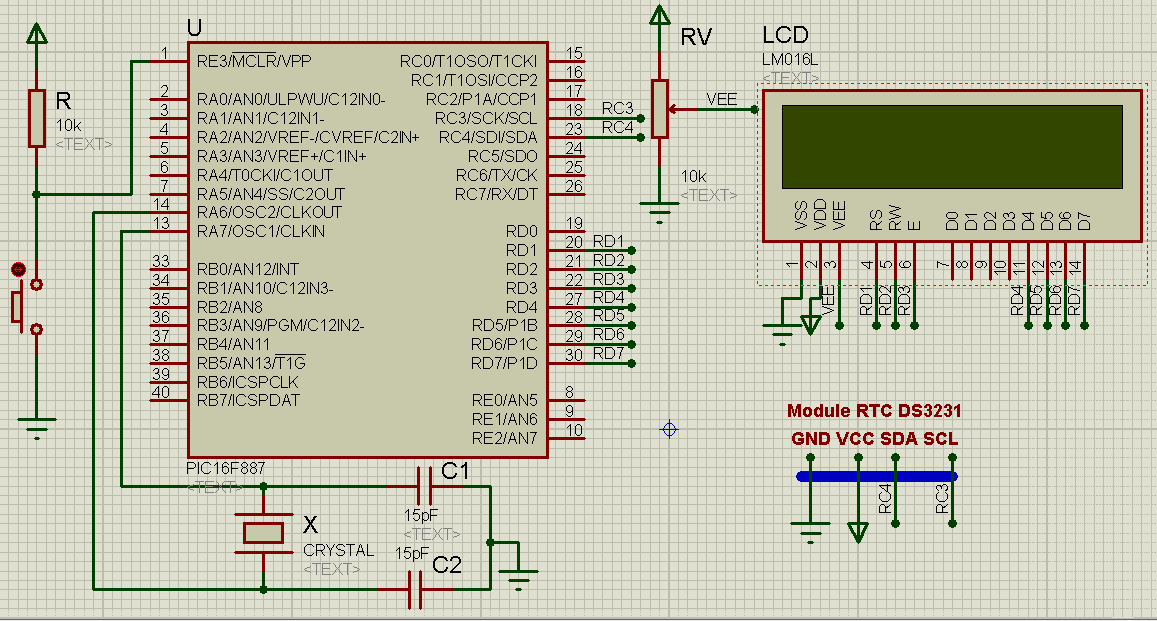
\includegraphics[scale=0.5]{bai-6/image/BAI-6-2}
\end{center}
\caption{Mạch đọc thời gian thực từ module RTC DS3231}
\end{figure}
\section*{Kết quả}
\begin{figure}[!h]
\begin{center}
%\subfloat[Sơ đồ mạch]
  {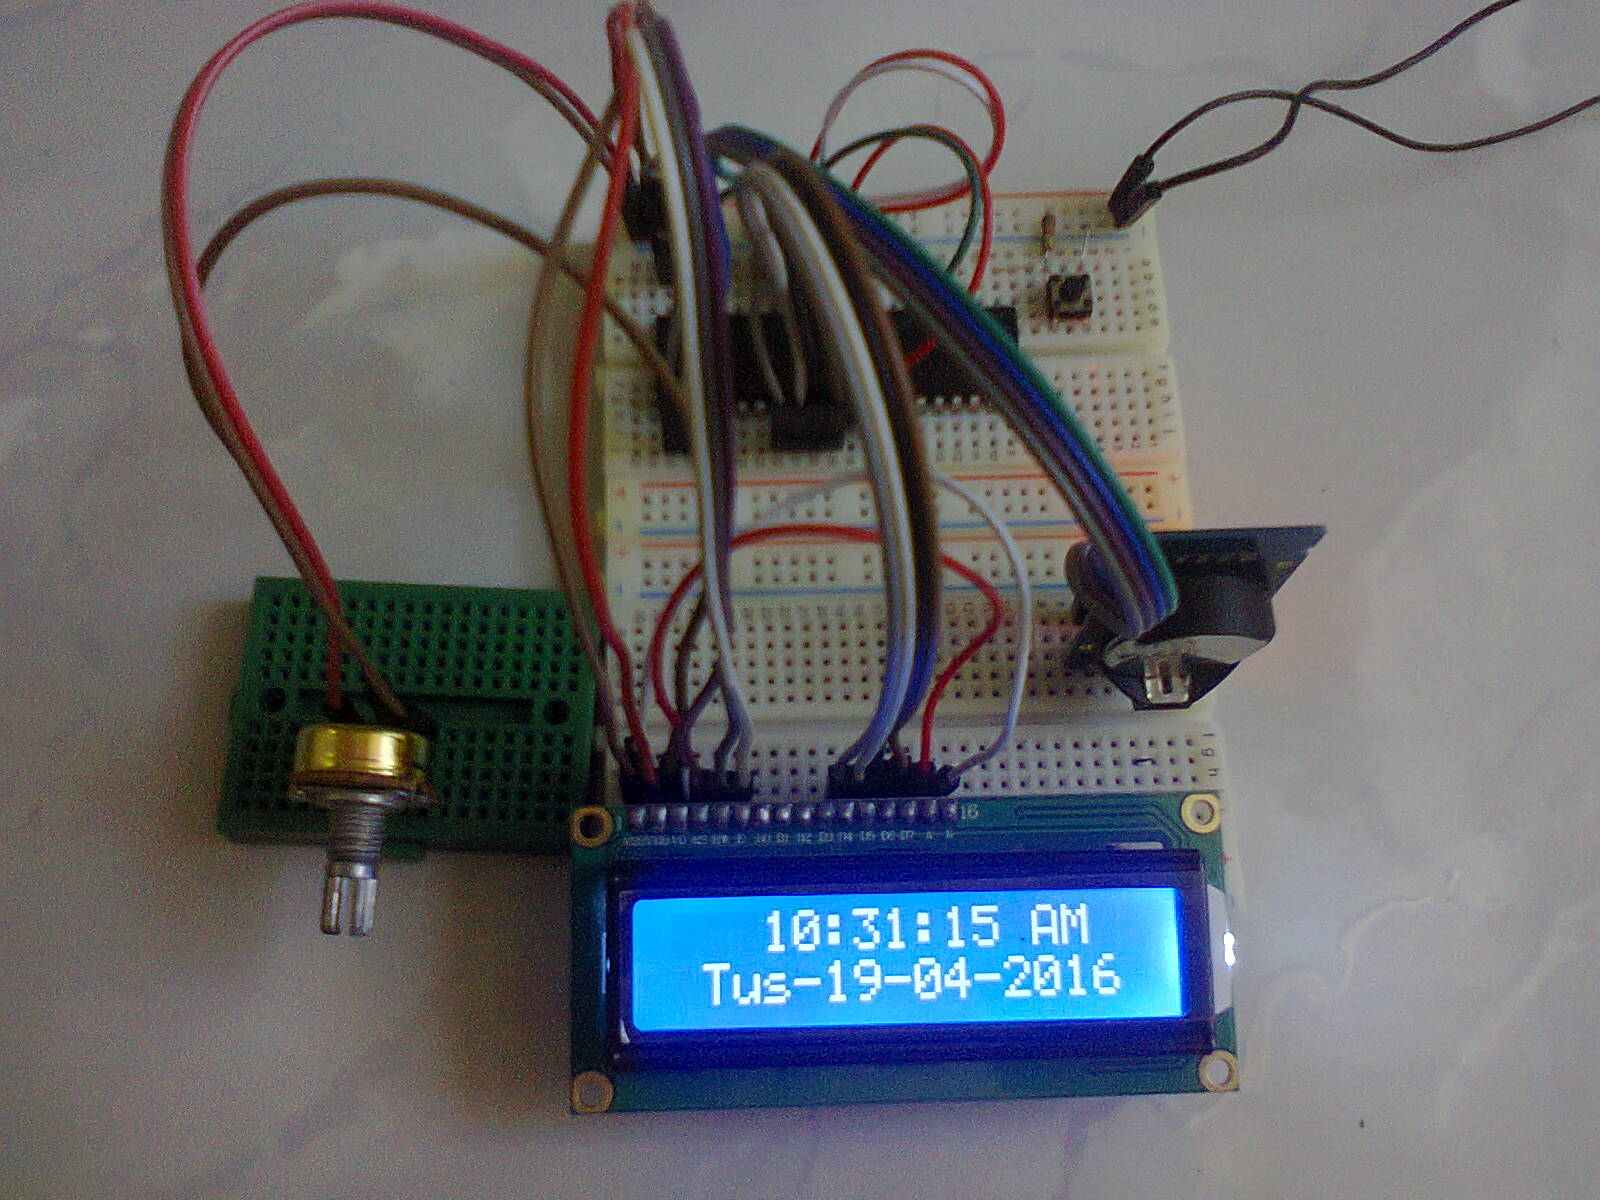
\includegraphics[width=.3\linewidth]{bai-6/image/6-2-1}}
%\subfloat[Kết quả]
  {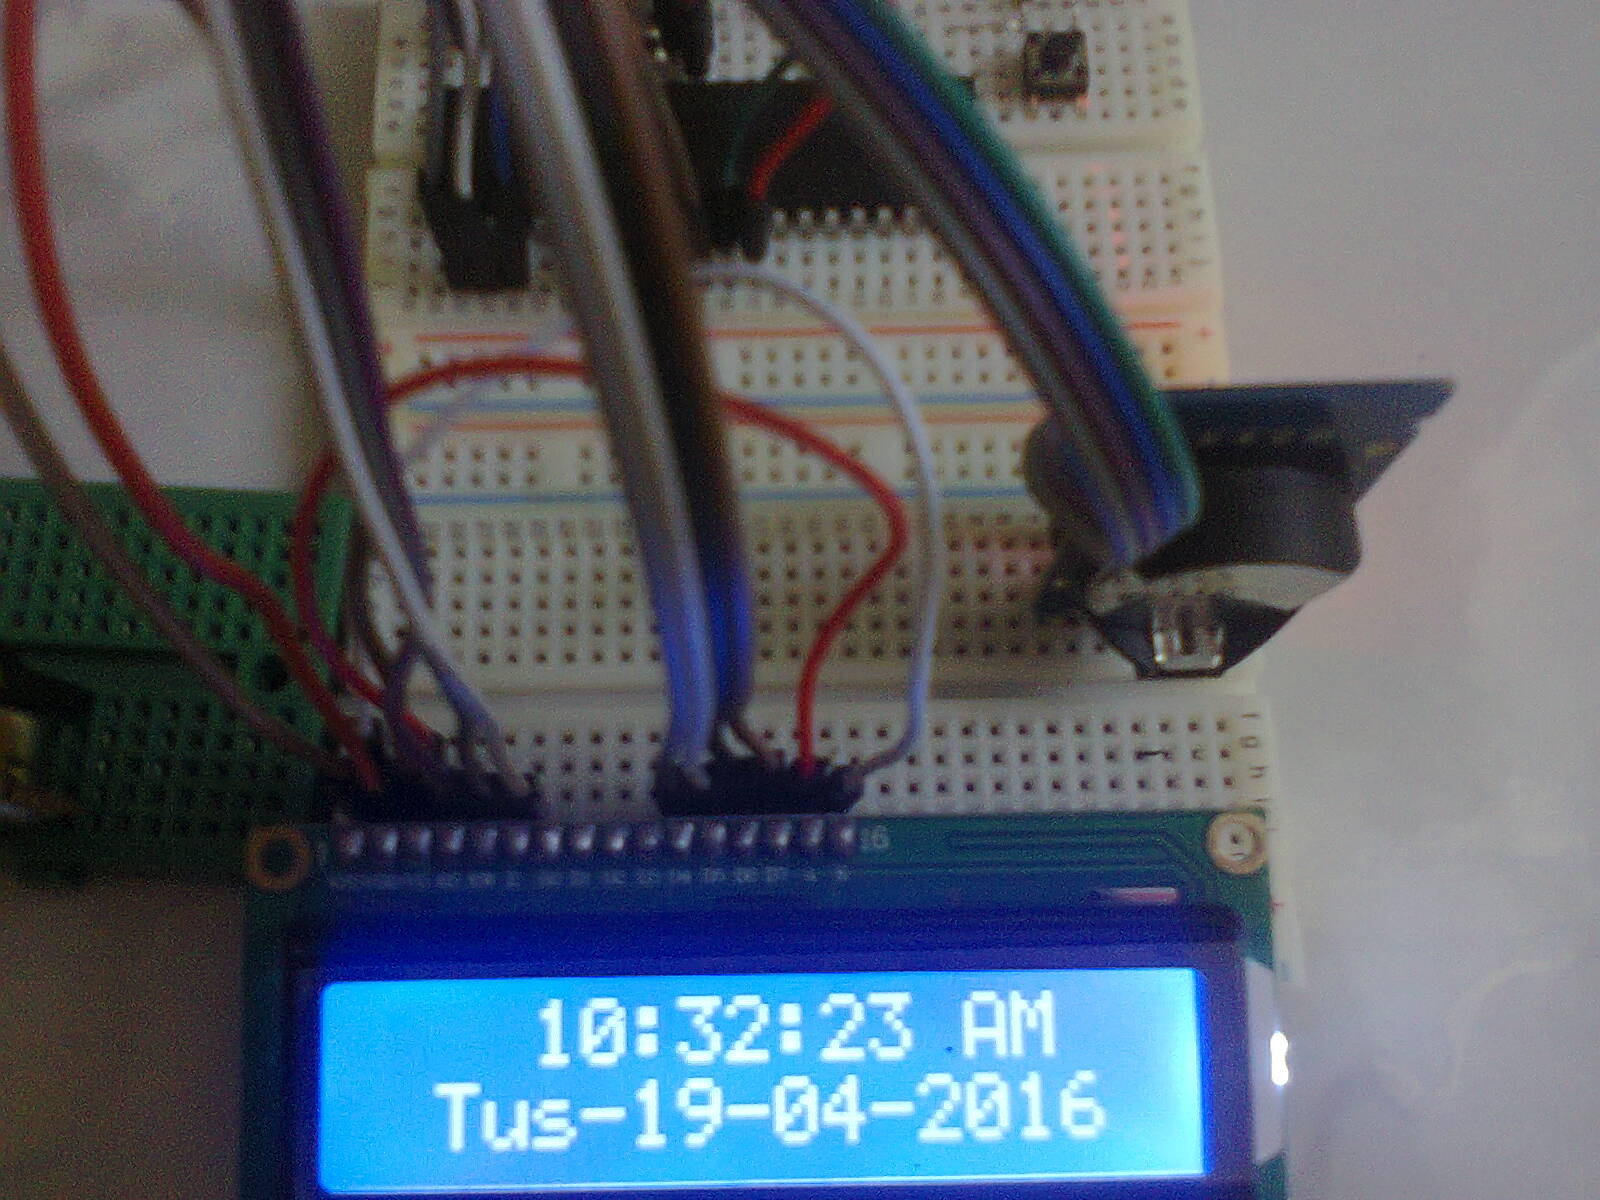
\includegraphics[width=.3\linewidth]{bai-6/image/6-2-2}}
  {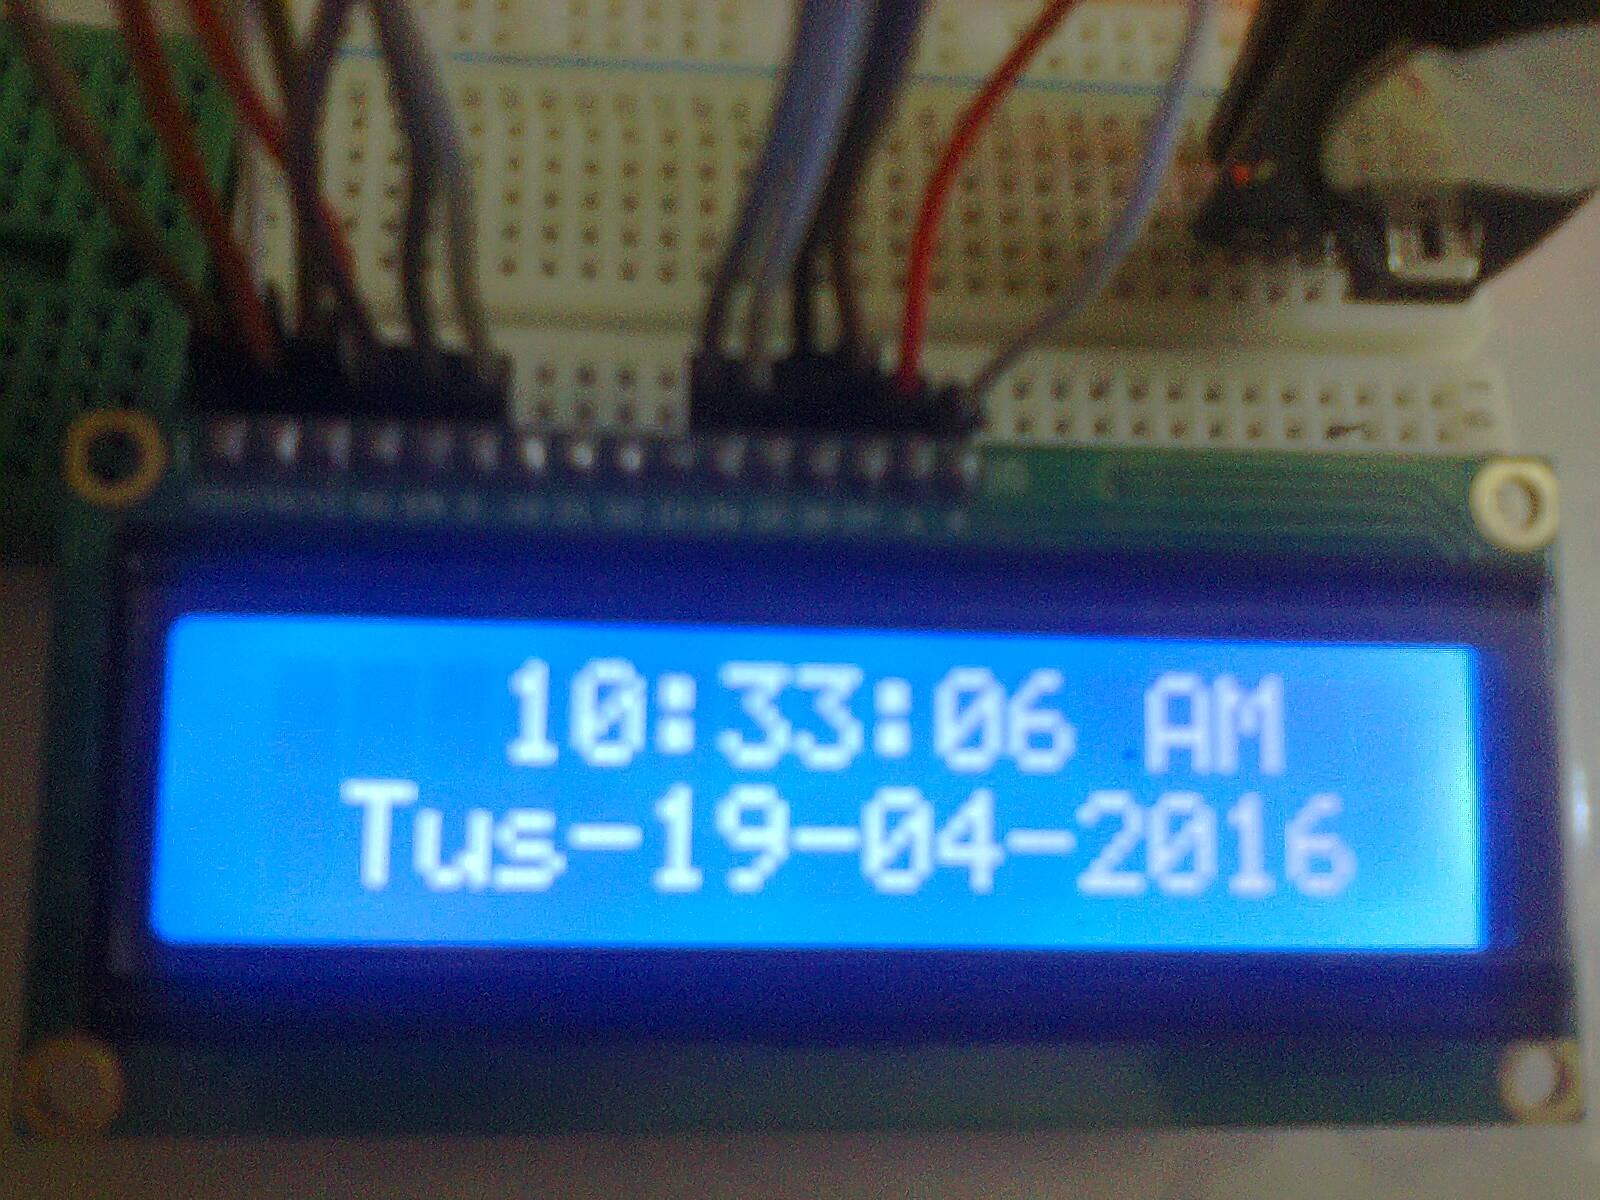
\includegraphics[width=.3\linewidth]{bai-6/image/6-2-3}}
\end{center}
\caption{Kết quả đọc thời gian thực từ IC DS3231}
\end{figure}
\subsection*{Chương trình 18 -- 1: Cài thời gian thực vào IC}
\lstinputlisting[language=C]{BAI-6-2-1.C}
\subsection*{Chương trình 18 -- 2: Lấy thời gian thực từ IC ra}
\lstinputlisting[language=C]{BAI-6-2-2.C}
\newpage
\subsection{Bài tập 6.3}
\label{Ex:ds3231-2}
\paragraph{Yêu cầu}Viết chương trình đồng hồ số hiển thị trên LCD 16x02 bao gồm giờ, phút, giây và nhiệt độ môi trường.
\paragraph{Hướng giải quyết}
\begin{itemize}
\item[$\ast$] Do sử dụng phần cứng là module RTC DS3231 nên ngoài chức năng lưu thời gian thực nó còn chức năng đọc nhiệt độ môi trường.
\item Địa chỉ của thanh ghi nhiệt độ là:
\begin{table}[!h]
\begin{center}
\begin{tabular}{|l|c|c|l|}\hline
\textit{Thanh ghi} & \textit{Địa chỉ} & \textit{Hàm} & \textit{Mô tả}\\ \hline
\verb|tempMSBREG| & \verb|0x11| & \verb|getTemp()| & Đọc vào nhiệt độ môi trường \\ \hline
\verb|tempLSBREG| & \verb|0x12| & & \\ \hline
\end{tabular}
\end{center}
\caption{IC DS3231 với chức năng đọc nhiệt độ môi trường}
\end{table}
\item Với phần thời gian thì chương trình giống như \textit{chương trình 18 -- 1} và \textit{chương trình 18 -- 2} của \textit{bài tập 6.2}. Phần nhiệt độ thì chúng ta thêm dòng lệnh sau vào vòng lặp \verb|while| và cho hiển thị giá trị đọc được lên LCD: \verb|getTemp();|
\end{itemize}
\paragraph{Sơ đồ mạch}Cách kết nối giống như \textit{bài tập 6.2}
\section*{Kết quả}
\begin{figure}[!h]
\begin{center}
%\subfloat[Sơ đồ mạch]
  {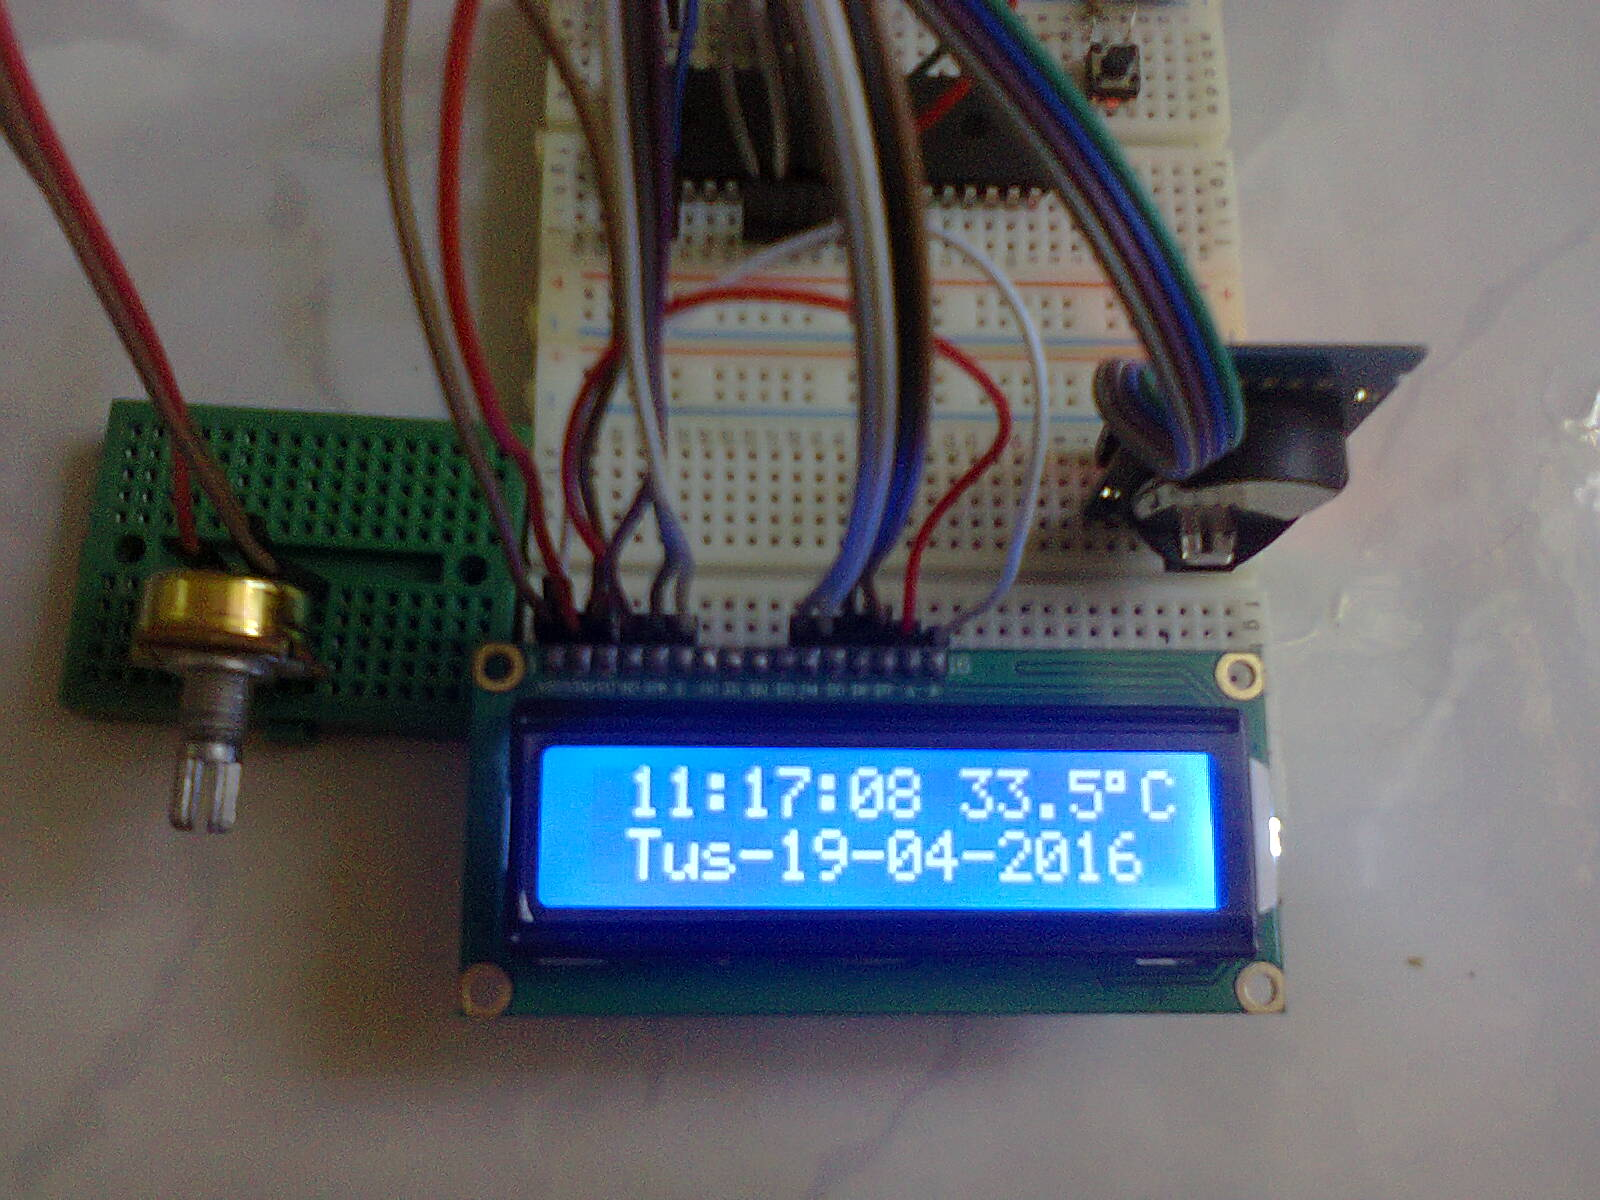
\includegraphics[width=.3\linewidth]{bai-6/image/6-3-1}}
%\subfloat[Kết quả]
  {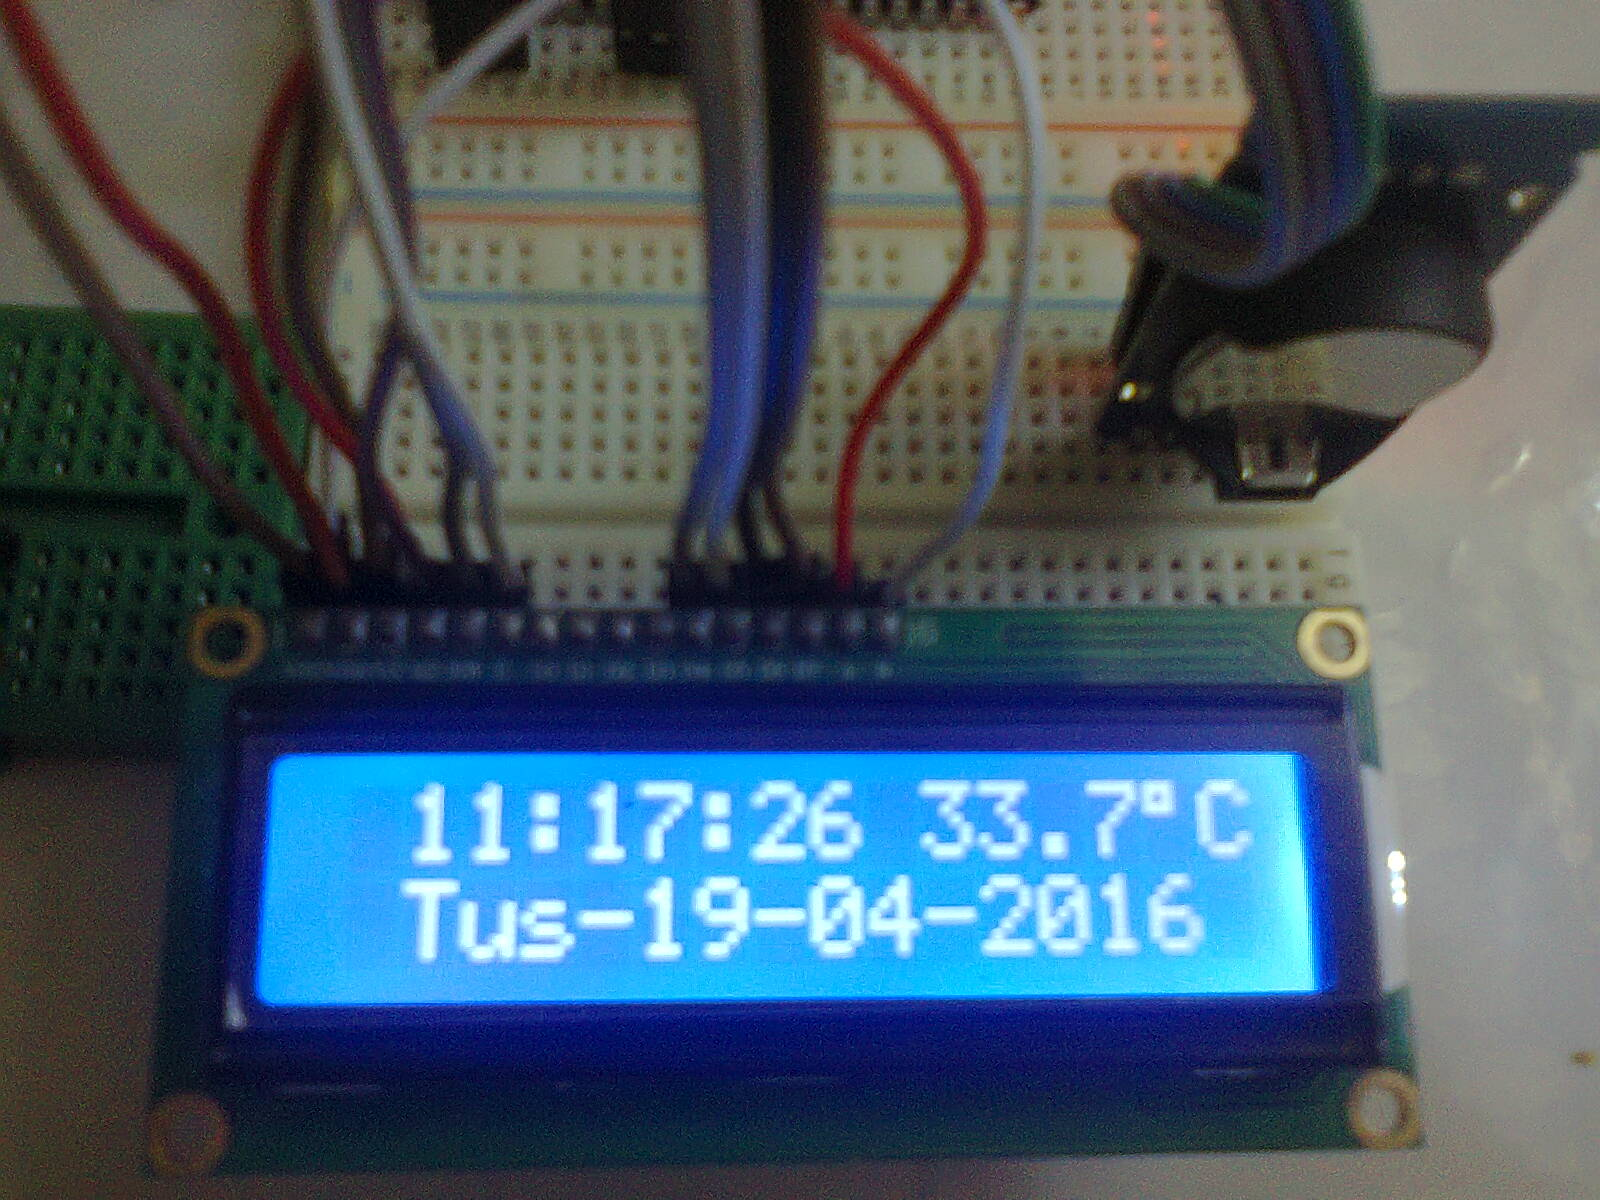
\includegraphics[width=.3\linewidth]{bai-6/image/6-3-2}}
  {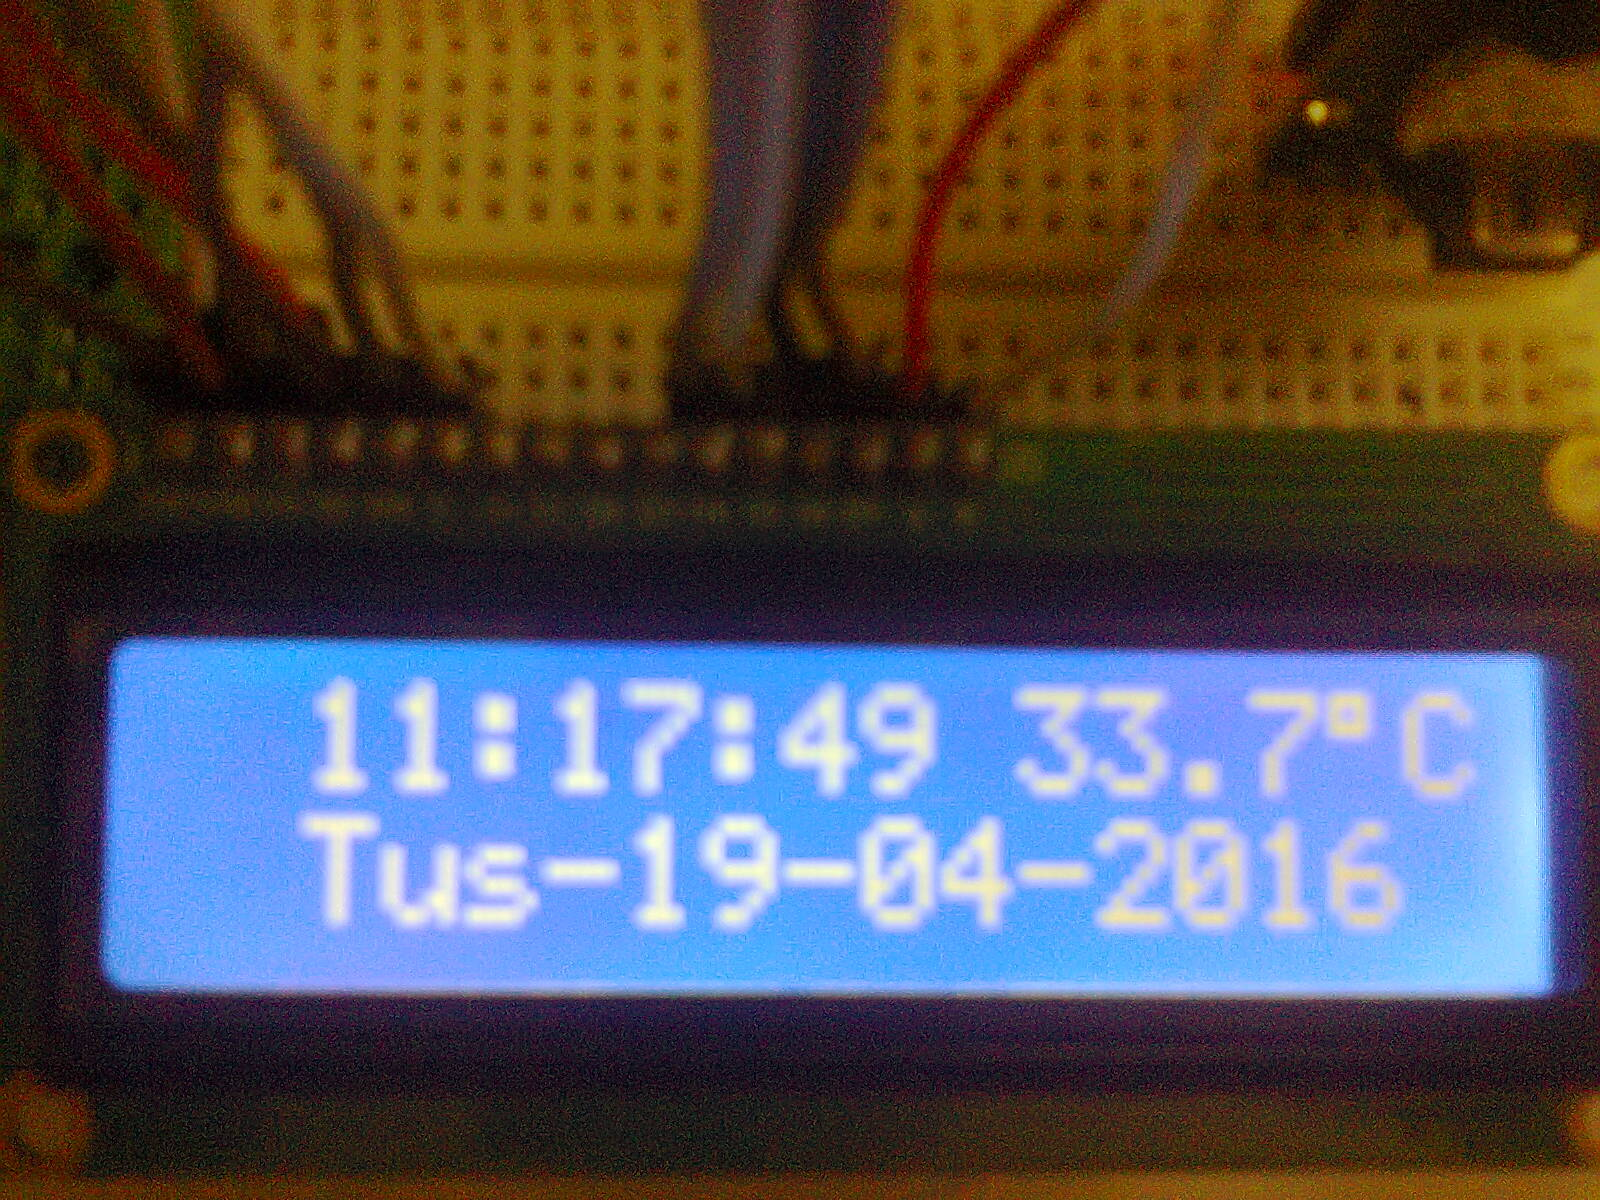
\includegraphics[width=.3\linewidth]{bai-6/image/6-3-3}}
\end{center}
\caption{Kết quả đọc thời gian thực  và nhiệt độ từ IC DS3231}
\end{figure}
\subsection*{Chương trình 19}
\label{code-19}
\lstinputlisting[language=C]{BAI-6-3.C}
\subsection{Mô phỏng cảm biến nhiệt TC74 với Protues}\label{def:TC74}
Trong quá trình tìm hiểu, em thấy có nhiều bạn gặp vấn đề khi mô phỏng cảm biến nhiệt độ TC74 với phần mềm protues. Em kiểm thử và tìm ra được là cảm biến nhiệt \verb|TC74| trong phần mềm mô phỏng \verb|Protues 7.8| nó tương thích với địa chỉ \verb|I2C| là \verb|0x9A| (đa phần các bạn làm trên địa chỉ \verb|0x90| nên khi mô phỏng thì ra giá trị nhiệt độ không đúng như đã cài đặt).

Về sơ đồ mạch và cách giải thích chương trình tương tự \textit{bài tập 6.1 trang \pageref{Ex:6-1}}.
\newpage
\paragraph{Chương trình sau mô phỏng được với phần mềm Protues 7.8}{~\\}
\lstinputlisting[language=C]{BAI-6-1V2.C}